\chapter{ROSDashboard: A Visual Debugging System for ROS}

[should the chapter be renamed to "prototype" or "prototypical implementation"?]

Write about rosdashboard (overview).

rosdashboard is a prototypical implementation of the system presented in \ref{visual_debugging_system} for the ROS middleware / framework. ROS was chosen as middleware because the simple publish/subscribe mechanism allowed to connect to topics transparently without the other party explicitly knowing about the visualization tool.

[Not sure if this is possible in other frameworks, if not it could be stated that more work is needed for those frameworks in order to make communication transparent. In general I can argue that ROS fits the requierements best, the system design was not intended to fit every framework but was developed without compromises current systems might have]

[I'm not sure how to write this chapter: can I have a section "why ROS?", "how the requirements are met?", ...?] ---> this should be written in the introduction for this chapter: ROS was used because it has many users, an easily accesible communication structure, a tool landscape (?) where such a tool would fit in well (recent surge of graphical tools like rxdeveloper, rqt, other dashboards).

\parbox{.8\linewidth}{
[from icra paper, needs some changes]

ROSDashboard, the tool presented in this work, aims to support the developer during debugging by visualizing data in a graphic way and thus eliminating the cognitive effort needed to parse and interpret text based logging messages. While most of the currently available visualization tools in robotics focus on spatial data to help understand the robot and the environment in which it runs \cite{Collett2010, Quigley2009}, rendering of abstract data is still uncommon. ROSDashboard provides a dashboard interface to robot developers, which they can populate with graphical widgets to visualize all kinds of data from the robot. The dashboard can be customized to display widgets according to the current robot hardware and development stage. It can be used to visualize data during debugging as well as monitor data during the normal execution of the robot. This means ROSDashboard is a tool that a) can be adapted to many different use cases and b) allows the developer to choose the widgets he or she thinks represent the data best, according to their mental model and the meaning of the data. The tool is based on ROS (Robot Operating System) which abstracts from specific robot hardware and takes care of inter process communication \cite{Quigley2009}.
}

\section{Related ROS Tools}
[list some tools and recent projects that have influenced the tool. For example the rxdeveloper tool and the survey in \cite{Muellers2012}, RQT and other dashboards recently developed. Highly related to the choice of makeing a tool for ros.]

\subsection{RQT - ROS GUI}
--> remove from debugging section, not related to debugging. can be introduced in rosdashboard when reasons for the choice of ros are presented (rosdashboard integrates well with other tools in the ros environment and recently many graphical tools were developed)

\subsection{rxDeveloper}
[\textbf{outline, results of the survey, importance for this work}]
\cite{Muellers2012}

[Not really debugging, this might go somewhere else? Maybe not a full subsecion but only a couple of sentences that summarize the results and why it is important for this work]


\section{Implementation Details}

\subsection{Visualization Widgets}
[List the currently available visualization, explain how to add new ones --> show that new widgets can be easily added]

\subsection{Topic Introspection}

\begin{figure}[thpb]
  \centering
  \framebox{
    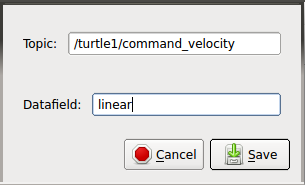
\includegraphics[scale=0.8]{img/topic_setup.png}
  }  
  \caption{Screenshot of the topic setup dialog. [re-do screenshot with rosdashboard in background]}
  \label{topic setup screenshot}
\end{figure}

ROS topics were originally not designed and developed as something the user or developer chooses graphically: They are usually created, configured and used in the source code. ROSDashboard exposes the topic setup in a graphical user interface every time a new widget is added to the dashboard. To make this as easy as possible and without much overhead, a technical solution was chosen to reduce the number of fields to be set during the topic subscription setup. Normally you have to select a topic name and a message data type. The data type can be one of the standard message types like Float, Integer, String and Boolean or a more complex message type which contains more information in a structured message. To access one data element of a message the ``datafield'' field was introduced in the graphical interface. Fig.~\ref{topic setup screenshot} shows an exemplary topic setup configuration to access the linear velocity of the \emph{/turtlesim/Velocity} message published to the topic \emph{/turtle1/command\_velocity}. Using Python's duck typing and the \emph{rostopic} module it was possible to avoid the complexity of dynamically binding message type classes during runtime and detect the message type automatically. If a topic is not yet published and thus the message type of this topic is not defined yet, the method call to \emph{rostopic} will block until the message type becomes available. To avoid blocking of the user interface a listener thread was implemented to wait until the message type for a topic becomes available (see Fig.~\ref{topic subscription}). Avoiding to manually ask the user for a message type makes the configuration of widgets easier and faster for the user, it also keeps the implementation significantly simpler, because no dynamic binding of message type classes during runtime is needed.

\begin{figure}[thpb]
  \centering
  \framebox{
    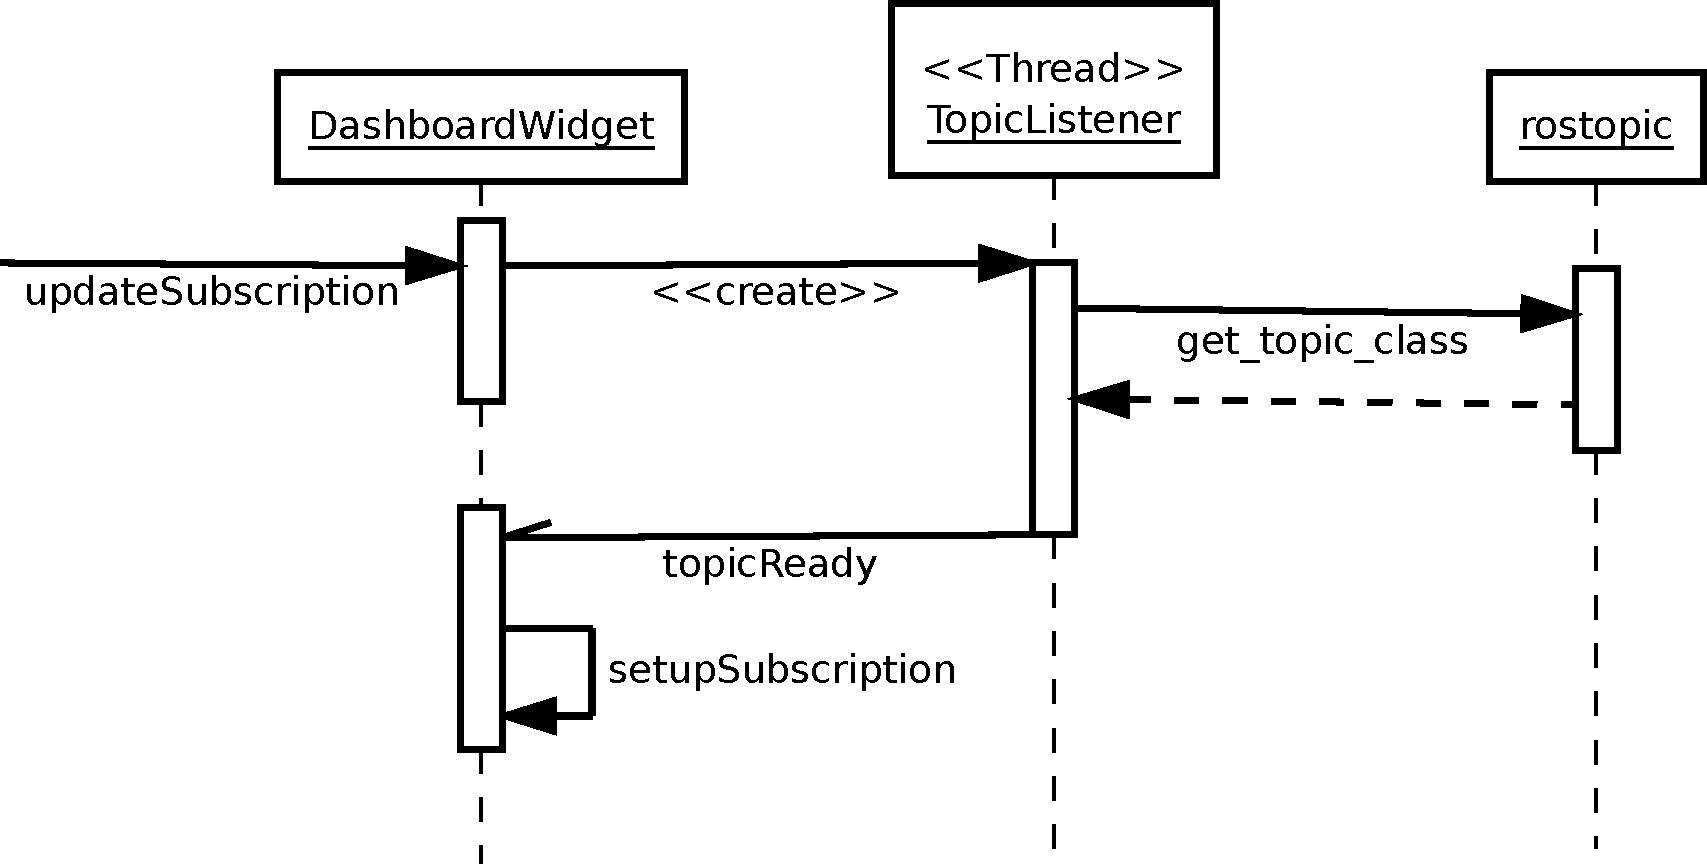
\includegraphics[scale=0.4]{diagrams/topic_subscription.pdf}
  }  
  \caption{Exemplary flow of events for asynchronous topic subscription setup.}
  \label{topic subscription}
\end{figure}

\subsection{User Interface}
[write about the user interface to configure widgets and the feature to delete widgets from the dashboard through drag and drop. should this be in the design?]

\subsection{Plugins}
Reference to the plugin framework section in \ref{visual_debugging_system} and that such a system was not yet implemented in ROSDashboard [can I say: due to the time constraints of this work?], but the necessary measures have been taken to allow this in the future. Show some details about an example widget and what methods it overwrites.
